\chapter{Case~Study: An~IDE~for~Research}

\sectionnote {BM}
\section {Overview}


\sectionnote {AC}
\section {Requirements}

Figures \ref{fig:case-research-use-case-project-management} through \ref{fig:case-research-use-case-project-workflow} display the individual use cases for the research IDE application. They have been separated into two diagrams based on workflow use cases and project management use cases.





TODO: WRITE MORE INFO HERE





\begin{figure}[!ht]
\centering 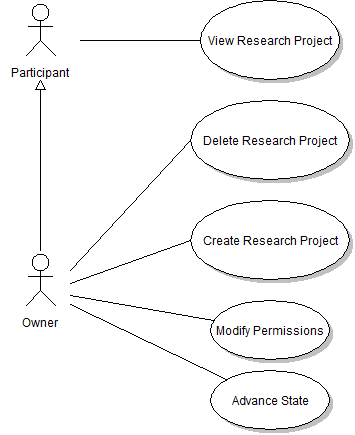
\includegraphics[height=5in]{./img/case-study-research-railgun/project_management_use_case}
\caption{Use case diagram for the project management functionality of the research IDE.}
\label{fig:case-research-use-case-project-management}
\end{figure}

\begin{figure}[!ht]
\centering 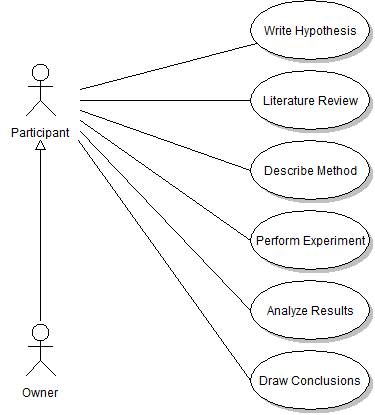
\includegraphics[height=5in]{./img/case-study-research-railgun/project_workflow_use_case}
\caption{Use case diagram for the project workflow functionality of the research IDE.}
\label{fig:case-research-use-case-project-workflow}
\end{figure}


Tables \ref{tbl:use-case-view-research-project} to \ref{tbl:use-case-draw-conclusions} provide the use case descriptions for the research IDE system. 
 

\begin{table}
  \centering
  \caption{Use case description for the ``View Research Project'' use case of the research IDE system.}
  \label{tbl:use-case-view-research-project}

  \begin{usecase}[View Research Project]
    \ucpart{Description}
    A User can view information about a project that he has permissions with.
    %
    \ucpart{Actors}
    Owner, Participant
    %
    \ucpart{Preconditions}
    The Research Project Exists and the User accessing it has at least one permission to view a task in the project.
    %
    \ucpart{Flow}
    \ucnormal
    \begin{ucenum}
      \item The User selects a research project from a list of projects that the User has access to.
      \item The User is shown detailed information about the project: current state of project, and any sections the user is allowed to view/edit.
    \end{ucenum}
    %
    \ucpart{Exceptions}
    \ucexception{No Permissions}
    The User has no permissions to view the project and is redirected back to a list of projects he has permission to view and an error is shown.
    %
    \ucpart{Postconditions}
    The User is brought to a details view of the selected project.
  \end{usecase}
\end{table}


\begin{table}
  \centering
  \caption{Use case description for the ``Delete Research Project'' use case of the research IDE system.}
  \label{tbl:use-case-delete-research-project}

  \begin{usecase}[Delete Research Project]
    \ucpart{Description}
    A Research Project can be deleted by the Owner of that project at any time.
    %
    \ucpart{Actors}
    Owner
    %
    \ucpart{Preconditions}
    The Research Project to be deleted exists.
    %
    \ucpart{Flow}
    \ucnormal
    \begin{ucenum}
      \item The User selects to delete the project.
      \item A confirmation box appears and the User agrees.
      \item The Project is deleted and the User is sent to a list of projects he has permission to view.
    \end{ucenum}
    %
    \ucpart{Variations}
    \ucbranch{A}
    \begin{ucenum}
      \item [A.2] A confirmation box appears and the User disagrees.
      \item [A.3] The User returns the the details view of that project.
    \end{ucenum}
    %
    \ucpart{Exceptions}
    \ucexception{Not Owner}
    A participant cannot delete a project he does not own. He is redirected back to the list of projects he has permission to view.
    %
    \ucpart{Postconditions}
    The Research Project is deleted from the system.
  \end{usecase}
\end{table}


\begin{table}
  \centering
  \caption{Use case description for the ``Create Research Project'' use case of the research IDE system.}
  \label{tbl:use-case-create-research-project}

  \begin{usecase}[Create Research Project]
    \ucpart{Description}
    A Research Project can be created by any User and that User becomes the Owner of that project.
    %
    \ucpart{Actors}
    Owner
    %
    \ucpart{Flow}
    \ucnormal
    \begin{ucenum}
      \item The User selects to Create a new Research Project.
      \item The User submits a name and description for the project.
      \item The Research project is created, The User is assigned as the owner and is redirected to viewing the project.
    \end{ucenum}
    %
    \ucpart{Postconditions}
    The Research Project is created and the User is assigned to the Owner of the project.
  \end{usecase}
\end{table}


\begin{table}
  \centering
  \caption{Use case description for the ``Modify Permissions'' use case of the research IDE system.}
  \label{tbl:use-case-modify-permissions}

  \begin{usecase}[Modify Permissions]
    \ucpart{Description}
    The Owner of a project can modify the permissions of other Users for his project.
    %
    \ucpart{Actors}
    Owner
    %
    \ucpart{Preconditions}
    The User is the Owner of the project to which he is assigned permissions.
    %
    \ucpart{Flow}
    \ucnormal
    \begin{ucenum}
      \item The User selects to modify the permissions for his project.
      \item A list of other Users on the system is shown along with their current.
      \item The User selects a specific permission to modify and submits the change.
      \item The other User now has the selected permissions for the project.
    \end{ucenum}
    %
    \ucpart{Exceptions}
    \ucexception{Cannot Modify Owner Permissions}
    The Owner always has every permission and this cannot be changed, redirected back to project view.
    \ucexception{Not Owner}
    Only Owners can modify permissions, redirected back to project view.
    %
    \ucpart{Postconditions}
    The User who had his permissions modified can now do any actions that require that permission.
  \end{usecase}
\end{table}


\begin{table}
  \centering
  \caption{Use case description for the ``Advance State'' use case of the research IDE system.}
  \label{tbl:use-case-advance-state}

  \begin{usecase}[Advance State]
    \ucpart{Description}
    The Owner can advance the state of the project as long as something has been saved into the current state.
    %
    \ucpart{Actors}
    Owner
    %
    \ucpart{Preconditions}
    There is another state in the workflow after the current state.
    %
    \ucpart{Flow}
    \ucnormal
    \begin{ucenum}
      \item The User selects to advance the state of the project
      \item There is something saved for the current state and the state is advanced to the next state in the workflow.
    \end{ucenum}
    %
    \ucpart{Variations}
    \ucbranch{A}
    \begin{ucenum}
      \item [A.2] There is nothing saved for the current state and a message is shown notifying the User that something must be saved before moving on.
    \end{ucenum}
    %
    \ucpart{Exceptions}
    \ucexception{Not Owner}
    A participant cannot advance the state of a project. He is redirected back to the project view
    \ucexception{Last State}
    There is no state after the current state so the state cannot be advanced, User is redirected back to project view.
    %
    \ucpart{Postconditions}
    The state of the workflow is advanced to the next state.
  \end{usecase}
\end{table}


\begin{table}
  \centering
  \caption{Use case description for the ``Write Hypothesis'' use case of the research IDE system.}
  \label{tbl:use-case-write-hypothesis}

  \begin{usecase}[Write Hypothesis]
    \ucpart{Description}
    A User with the correct permissions can edit or view the hypothesis of the current project.
    %
    \ucpart{Actors}
    Owner, Participant
    %
    \ucpart{Preconditions}
    The workflow must be in the ‘Write Hypothesis”, “Literature Review” or “Describe Method” state. The User has the ‘edit’ or ‘view’ permission for this task.
    %
    \ucpart{Flow}
    \ucnormal
    \begin{ucenum}
      \item The User selects to write the hypothesis.
      \item The User has the ‘edit’ permission and makes a modification to the hypothesis and selects to save.
      \item The Hypothesis is updated and saved.
    \end{ucenum}
    %
    \ucpart{Variations}
    \ucbranch{A}
    \begin{ucenum}
      \item [A.2] The User has the ‘view’ permission and does not have the ‘edit’ permission and is shown the current hypothesis.
    \end{ucenum}
    %
    \ucpart{Exceptions}
    \ucexception{No Permission}
    The User does not have permission to ‘edit’ or ‘view’ the hypothesis and is returned to project view.
  \end{usecase}
\end{table}


\begin{table}
  \centering
  \caption{Use case description for the ``Literature Review'' use case of the research IDE system.}
  \label{tbl:use-case-literature-review}

  \begin{usecase}[Literature Review]
    \ucpart{Description}
    A User with the correct permissions can edit or view the literature review of the current project.
    %
    \ucpart{Actors}
    Owner, Participant
    %
    \ucpart{Preconditions}
    The workflow must be in the “Literature Review” or “Describe Method” state. The User has the ‘edit’ or ‘view’ permission for this task.
    %
    \ucpart{Flow}
    \ucnormal
    \begin{ucenum}
      \item The User selects to work on the literature review.
      \item The User has the ‘edit’ permission and makes a modification to the literature review and selects to save.
      \item The Literature Review is updated and saved.
    \end{ucenum}
    %
    \ucpart{Variations}
    \ucbranch{A}
    \begin{ucenum}
      \item [A.2] The User has the ‘view’ permission and does not have the ‘edit’ permission and is shown the current literature review.
    \end{ucenum}
    %
    \ucpart{Exceptions}
    \ucexception{No Permission}
    The User does not have permission to ‘edit’ or ‘view’ the literature review and is returned to project view.
  \end{usecase}
\end{table}


\begin{table}
  \centering
  \caption{Use case description for the ``Describe Method'' use case of the research IDE system.}
  \label{tbl:use-case-describe-method}

  \begin{usecase}[Describe Method]
    \ucpart{Description}
    A User with the correct permissions can edit or view the method of the selected project.
    %
    \ucpart{Actors}
    Owner, Participant
    %
    \ucpart{Preconditions}
    The workflow is in the “Describe Method” state. The User has the ‘edit’ or ‘view’ permission for this task.
    %
    \ucpart{Flow}
    \ucnormal
    \begin{ucenum}
      \item The User selects to describe the method of the experiment.
      \item The User has the ‘edit’ permission and makes a modification to the method and selects to save.
      \item The Method is updated and saved to the system.
    \end{ucenum}
    %
    \ucpart{Variations}
    \ucbranch{A}
    \begin{ucenum}
      \item [A.2] The User has the ‘view’ permission and does not have the ‘edit’ permission and is shown the current method.
    \end{ucenum}
    %
    \ucpart{Exceptions}
    \ucexception{No Permission}
    The User does not have permission to ‘edit’ or ‘view’ the method and is returned to project view.
  \end{usecase}
\end{table}


\begin{table}
  \centering
  \caption{Use case description for the `'Perform Experiment'' use case of the research IDE system.}
  \label{tbl:use-case-perform-experiment}

  \begin{usecase}[Perform Experiment]
    \ucpart{Description}
    A User with correct permissions selects to perform the experiment. This closes the ability to make modifications to the hypothesis and the method  and allows experimental data to be entered.
    %
    \ucpart{Actors}
    Owner, Participant
    %
    \ucpart{Preconditions}
    The workflow must be in the “Perform Experiment” state. The User has the ‘edit’ or ‘view’ permission for this task.
    %
    \ucpart{Flow}
    \ucnormal
    \begin{ucenum}
      \item The User selects to perform the experiment.
      \item The User has the ‘edit’ permission and makes a modification to the experimental data and selects to save.
      \item The experimental data is updated and saved to the system.
    \end{ucenum}
    %
    \ucpart{Variations}
    \ucbranch{A}
    \begin{ucenum}
      \item [A.2] The User has the ‘view’ permission and does not have the ‘edit’ permission and is shown the current experimental data.
    \end{ucenum}
    %
    \ucpart{Exceptions}
    \ucexception{No Permission}
    The User does not have permission to ‘edit’ or ‘view’ the experimental data and is returned to project view.
  \end{usecase}
\end{table}


\begin{table}
  \centering
  \caption{Use case description for the `'Analyze Results'' use case of the research IDE system.}
  \label{tbl:use-case-analyze-results}

  \begin{usecase}[Analyze Results]
    \ucpart{Description}
    A User with correct permissions selects to analyze the results of the experiment.
    %
    \ucpart{Actors}
    Owner, Participant
    %
    \ucpart{Preconditions}
    The workflow must be in the “Analyze Results” state. The User has the ‘edit’ or ‘view’ permission for this task.
    %
    \ucpart{Flow}
    \ucnormal
    \begin{ucenum}
      \item The User selects to analyze the results of the experiment.
      \item The User has the ‘edit’ permission and makes a modification to the analysis and selects to save.
      \item The analysis is updated and saved to the system.
    \end{ucenum}
    %
    \ucpart{Variations}
    \ucbranch{A}
    \begin{ucenum}
      \item [A.2] The User has the ‘view’ permission and does not have the ‘edit’ permission and is shown the current analysis.
    \end{ucenum}
    %
    \ucpart{Exceptions}
    \ucexception{No Permission}
    The User does not have permission to ‘edit’ or ‘view’ the analysis and is returned to project view.
  \end{usecase}
\end{table}


\begin{table}
  \centering
  \caption{Use case description for the `'Draw Conclusions'' use case of the research IDE system.}
  \label{tbl:use-case-draw-conclusions}

  \begin{usecase}[Draw Conclusions]
    \ucpart{Description}
    A User with correct permissions selects to draw conclusions.
    %
    \ucpart{Actors}
    Owner, Participant
    %
    \ucpart{Preconditions}
    The workflow must be in the “Draw Conclusions” state. The User has the ‘edit’ or ‘view’ permission for this task.
    %
    \ucpart{Flow}
    \ucnormal
    \begin{ucenum}
      \item The User selects to draw conclusions for the project.
      \item The User has the ‘edit’ permission and makes a modification to the conclusion and selects to save.
      \item The conclusion is updated and saved to the system.
    \end{ucenum}
    %
    \ucpart{Variations}
    \ucbranch{A}
    \begin{ucenum}
      \item [A.2] The User has the ‘view’ permission and does not have the ‘edit’ permission and is shown the current conclusion.
    \end{ucenum}
    %
    \ucpart{Exceptions}
    \ucexception{No Permission}
    The User does not have permission to ‘edit’ or ‘view’ the conclusion and is returned to project view.
  \end{usecase}
\end{table}


\sectionnote {BM}
\section {Design}
